\documentclass[twoside]{article}

\usepackage{lipsum}
\usepackage{graphicx}
\usepackage{placeins}

\usepackage[utf8]{inputenc}
\usepackage[T1]{fontenc}
\usepackage[sc]{mathpazo} % Palatino
\usepackage[brazil]{babel}
\linespread{1.15}
\usepackage{microtype}

\usepackage[hmarginratio=1:1,top=32mm,columnsep=20pt]{geometry}
\usepackage{multicol}
\usepackage[hang, small,labelfont=bf,up,textfont=it,up]{caption}
\usepackage{booktabs}
\usepackage{float}
\usepackage{hyperref}

\usepackage{lettrine}
\usepackage{paralist}

\usepackage{abstract}
\renewcommand{\abstractnamefont}{\normalfont\bfseries}
\renewcommand{\abstracttextfont}{\normalfont\small\itshape}

\usepackage{titlesec}
\setcounter{secnumdepth}{2}
% Seção: sem número no título
\titleformat{\section}[block]{\large\bfseries}{}{0em}{}

% Formato do número da subseção: seção.subseção → 1.0, 1.1, 2.0...
\renewcommand\thesubsection{\arabic{subsection}{.}\arabic{subsubsection}}

% Subseção: mostra o número (1.0, 1.1, ...) e o título em negrito
\titleformat{\subsection}[block]{\large\bfseries}{\thesubsection}{1em}{}


\usepackage{fancyhdr}
\pagestyle{fancy}
\fancyhead{}
\fancyfoot{}
\fancyhead[C]{Running title $\bullet$ November 2025 $\bullet$ Vol. XXI, No. 1}
\fancyfoot[RO,LE]{\thepage}

% Citações ABNT autor-data
\usepackage[alf]{abntex2cite}

%----------------------------------------------------------------------------------------
%   TÍTULO E AUTORES (CENTRALIZADOS)
%----------------------------------------------------------------------------------------

% Redefine o \maketitle para centralizar título e autores
\makeatletter
\renewcommand{\maketitle}{%
  \begin{center}
    {\fontsize{24pt}{10pt}\selectfont\bfseries \@title\par}%
    \vspace{1em}
    {\large \@author\par}%
    \vspace{1em}
  \end{center}
}
\makeatother

\title{
	Computação Neuromórfica e Redes Neurais para Predição da Qualidade da Água em Ambientes Amazônicos
}

\author{%
	Felipe de Vasconcelos Assunção\textsuperscript{1},
	Alfredo Paulo\textsuperscript{1},
	Aluno 1\textsuperscript{1},
	Vandermi João da Silva\textsuperscript{1},
	Professor Alex\textsuperscript{1}\\[2mm]
	\textsuperscript{1}Universidade Federal do Amazonas (UFAM)\\[1mm]
	\texttt{felipe.assuncao@ufam.edu.br, alfredo.paulo@ufam.edu.br,}\\
	\texttt{aluno@ufam.edu.br, vandermi.silva@ufam.edu.br, alex@ufam.edu.br}%
}

\date{}

%----------------------------------------------------------------------------------------

\begin{document}

\maketitle
\thispagestyle{fancy}

%----------------------------------------------------------------------------------------
%   ABSTRACT
%----------------------------------------------------------------------------------------

\begin{abstract}
	\noindent
	O monitoramento da qualidade da água na Bacia Amazônica é um desafio logístico e
	operacional devido à sua vasta extensão territorial e infraestrutura limitada.
	Este artigo investiga a viabilidade da implementação de Redes Neurais Pulsadas (SNNs)
	em microcontroladores de baixo custo para a predição de parâmetros da qualidade da água,
	visando otimizar o consumo energético e a autonomia dos dispositivos de monitoramento
	remoto. A pesquisa propõe uma abordagem quantitativa, utilizando dados coletados no Lago 
	do Serpa, em Itacoatiara - AM, para avaliar o desempenho preditivo das SNNs aplicadas a 
	variáveis físico-químicas como pH, turbidez e oxigênio dissolvido. Os resultados esperados
	incluem a identificação dos parâmetros mais sensíveis à modelagem com SNNs, bem como a
	validação da eficácia do modelo em cenários reais, contribuindo para o avanço das
	tecnologias de monitoramento ambiental na região amazônica.
\end{abstract}

%----------------------------------------------------------------------------------------
%   OBJETIVOS
%----------------------------------------------------------------------------------------

\subsection{Objetivo Geral}

Avaliar a viabilidade de algoritmos de Redes Neurais Pulsadas (SNNs), baseados em princípios da 
computação neuromórfica e implementados em microcontroladores de baixo custo, para a classificação e 
predição espaço-temporal da qualidade da água, com foco na identificação e expansão de manchas 
de poluição em ambientes amazônicos.

\subsection{Objetivos Específicos}

\begin{compactitem}
  \item Verificar a capacidade de microcontroladores de baixo custo em executar 
  modelos de Redes Neurais Pulsadas (SNNs) com desempenho computacional adequado 
  para aplicações ambientais na Amazônia.

  \item Identificar os parâmetros físico-químicos da qualidade da água mais sensíveis 
  à modelagem com SNNs, considerando dados coletados no Lago do Serpa.

  \item Analisar o comportamento temporal e espacial dos dados de qualidade da água, 
  visando à caracterização da distribuição da mancha de poluição no ambiente 
  aquático estudado.

  \item Classificar a qualidade da água do Lago do Serpa a partir dos parâmetros 
  físico-químicos preditos, de modo a delimitar espacialmente a mancha de poluição.

  \item Avaliar o desempenho das SNNs em relação a algoritmos tradicionais de 
  aprendizado de máquina aplicados em microcontroladores, considerando métricas 
  de acurácia, tempo de inferência e consumo energético.

  \item Validar a capacidade dos modelos neuromórficos em prever a expansão 
  espaço-temporal da mancha de poluição, utilizando séries temporais de dados 
  reais da região amazônica.
\end{compactitem}



%----------------------------------------------------------------------------------------
%   REFERENCIAL TEÓRICO
%----------------------------------------------------------------------------------------
\FloatBarrier
\section{REFERENCIAL TEÓRICO}

A evolução dos sistemas de monitoramento ambiental tem migrado
consistentemente de abordagens reativas e baseadas em amostragem
pontual para modelos preditivos contínuos e baseados em dados massivos.
\citeonline{zulkifli2022} realizaram uma revisão sistemática abrangente
demonstrando que a arquitetura IoT se consolidou como a espinha dorsal
para a aquisição de dados em tempo real de parâmetros físico-químicos
essenciais, como pH, turbidez, oxigênio dissolvido e temperatura.
A recente integração de agentes autônomos de IA a esses ecossistemas
de IoT permite não apenas a leitura passiva de sensores, mas a
interpretação ativa e autônoma de padrões complexos, não lineares e
multivariados inerentes aos corpos hídricos, possibilitando a detecção
de anomalias sutis que passariam despercebidas por métodos convencionais
\cite{miller2025}.

No domínio específico dos algoritmos de aprendizado de máquina aplicados
à hidrologia, \citeonline{yan2024} analisaram a literatura dos últimos cinco
anos e identificaram que modelos de Deep Learning, especificamente as
Redes Neurais Recorrentes (RNN) e suas variantes modernas como LSTM e GRU,
superam consistentemente métodos estatísticos clássicos e modelos de
Machine Learning tradicionais (como SVM e Random Forest) na previsão de
qualidade da água. Essa superioridade deve-se à capacidade intrínseca dessas
redes de reter memórias de longo prazo e capturar dependências temporais complexas
em séries hidrológicas. \citeonline{liu2019} corroboram essa visão, demonstrando a
aplicação bem-sucedida de LSTMs para corrigir falhas em sensores, imputar dados
faltantes e prever tendências futuras em ambientes de IoT sujeitos a ruídos e
interrupções.

Além disso, \citeonline{wu2022} destacam que modelos híbridos, que
combinam técnicas de pré-processamento de sinal avançadas, como a
Transformada Wavelet, com redes LSTMs, oferecem uma robustez ainda maior
contra ruídos de alta frequência e artefatos, comuns em sensores de campo
operando em condições adversas.
\citeonline{pan2022} reforçam essa perspectiva ao revisar os avanços recentes
na combinação de sensoriamento remoto e IA para previsão de qualidade da
água em rios, enfatizando a importância de abordagens integradas para
lidar com a variabilidade espacial e temporal desses ecossistemas.
Da mesma forma, \citeonline{ahmed2019} argumentam que métodos de aprendizado
de máquina, quando bem calibrados, superam significativamente abordagens
tradicionais em termos de precisão preditiva.

Entretanto, a transição desses modelos avançados de ambientes controlados
para a implementação em hardware restrito na borda (Edge AI) impõe
barreiras técnicas significativas.
\citeonline{elshafeiy2023} e \citeonline{lamrini2024} discutem extensivamente
a necessidade crítica de desenvolver algoritmos leves e eficientes para a
detecção de anomalias in situ, visando reduzir drasticamente o tráfego de
dados via redes sem fio e, consequentemente, o consumo de energia do
sistema.
\citeonline{aladhaileh2021} também apontam para a importância de modelos
preditivos eficientes para a gestão sustentável de recursos hídricos.
\citeonline{chadalavada2025} propuseram recentemente as Gated Liquid Neural
Networks (Gated-LNN) como uma evolução arquitetural para lidar melhor com
a irregularidade e a natureza assíncrona dos dados de sensores
ambientais, mas ainda operando dentro do paradigma de redes neurais de
ativação contínua.

Por outro lado, a computação neuromórfica baseada em SNNs oferece uma
mudança fundamental de paradigma.
Ao operar com base em eventos discretos e comunicação por spikes, o
consumo de energia nessas redes torna-se proporcional à atividade do
sinal de entrada, e não à frequência de clock do processador.
Essa característica é ideal para o monitoramento de parâmetros
ambientais que frequentemente permanecem estáveis por longos períodos,
mas que exigem detecção instantânea e precisa de mudanças bruscas
indicativas de eventos de contaminação ou desastres naturais.
\citeonline{alprol2024} discutem como tecnologias de IA estão
revolucionando o tratamento de águas residuais, e princípios similares
podem ser aplicados ao monitoramento ambiental na Amazônia.
Finalmente, \citeonline{qi2020} demonstram a eficácia de modelos
LSTM-RNN combinados com sensoriamento remoto para monitoramento de
qualidade da água em grandes corpos hídricos, fornecendo uma base sólida
para a comparação com as SNNs propostas.

\FloatBarrier
\subsection{Lócus da Pesquisa}

O lócus desta pesquisa é a comunidade quilombola Sagrado Coração de Jesus do Lago do Serpa,
localizada no município de Itacoatiara, Amazonas. Esta comunidade tradicional, certificada 
pela Fundação Cultural Palmares em 2004, habita as margens do Lago do Serpa, um importante 
corpo hídrico de várzea \cite{clemente2018}. A escolha deste local justifica-se por 
sua representatividade socioambiental e pelos desafios logísticos inerentes à 
região amazônica.

Historicamente, o quilombo formou-se a partir de famílias de negros remanescentes
que buscavam refúgio e autonomia, mantendo até hoje laços estreitos com o território
e seus recursos naturais \cite{nogueira2022}. O Lago do Serpa não é apenas 
um recurso hídrico, mas um elemento central na vida da comunidade, servindo para pesca, 
transporte e lazer, além de possuir significado cultural e identitário profundo 
\cite{clemente2018}. No entanto, a comunidade enfrenta desafios contemporâneos 
relacionados à preservação ambiental e à garantia de qualidade de vida, o que torna o 
monitoramento da qualidade da água uma questão de saúde pública e justiça ambiental 
\cite{nogueira2022}. A dinâmica hidrológica do lago, sujeita ao pulso de 
inundação do Rio Amazonas e à pressão antrópica local, oferece um cenário complexo e 
ideal para testar a robustez de sistemas de monitoramento baseados em IA.

\begin{figure}[ht!] 
    \centering
	\caption{Lago de Serpa -- Itacoatiara, Amazonas.}
    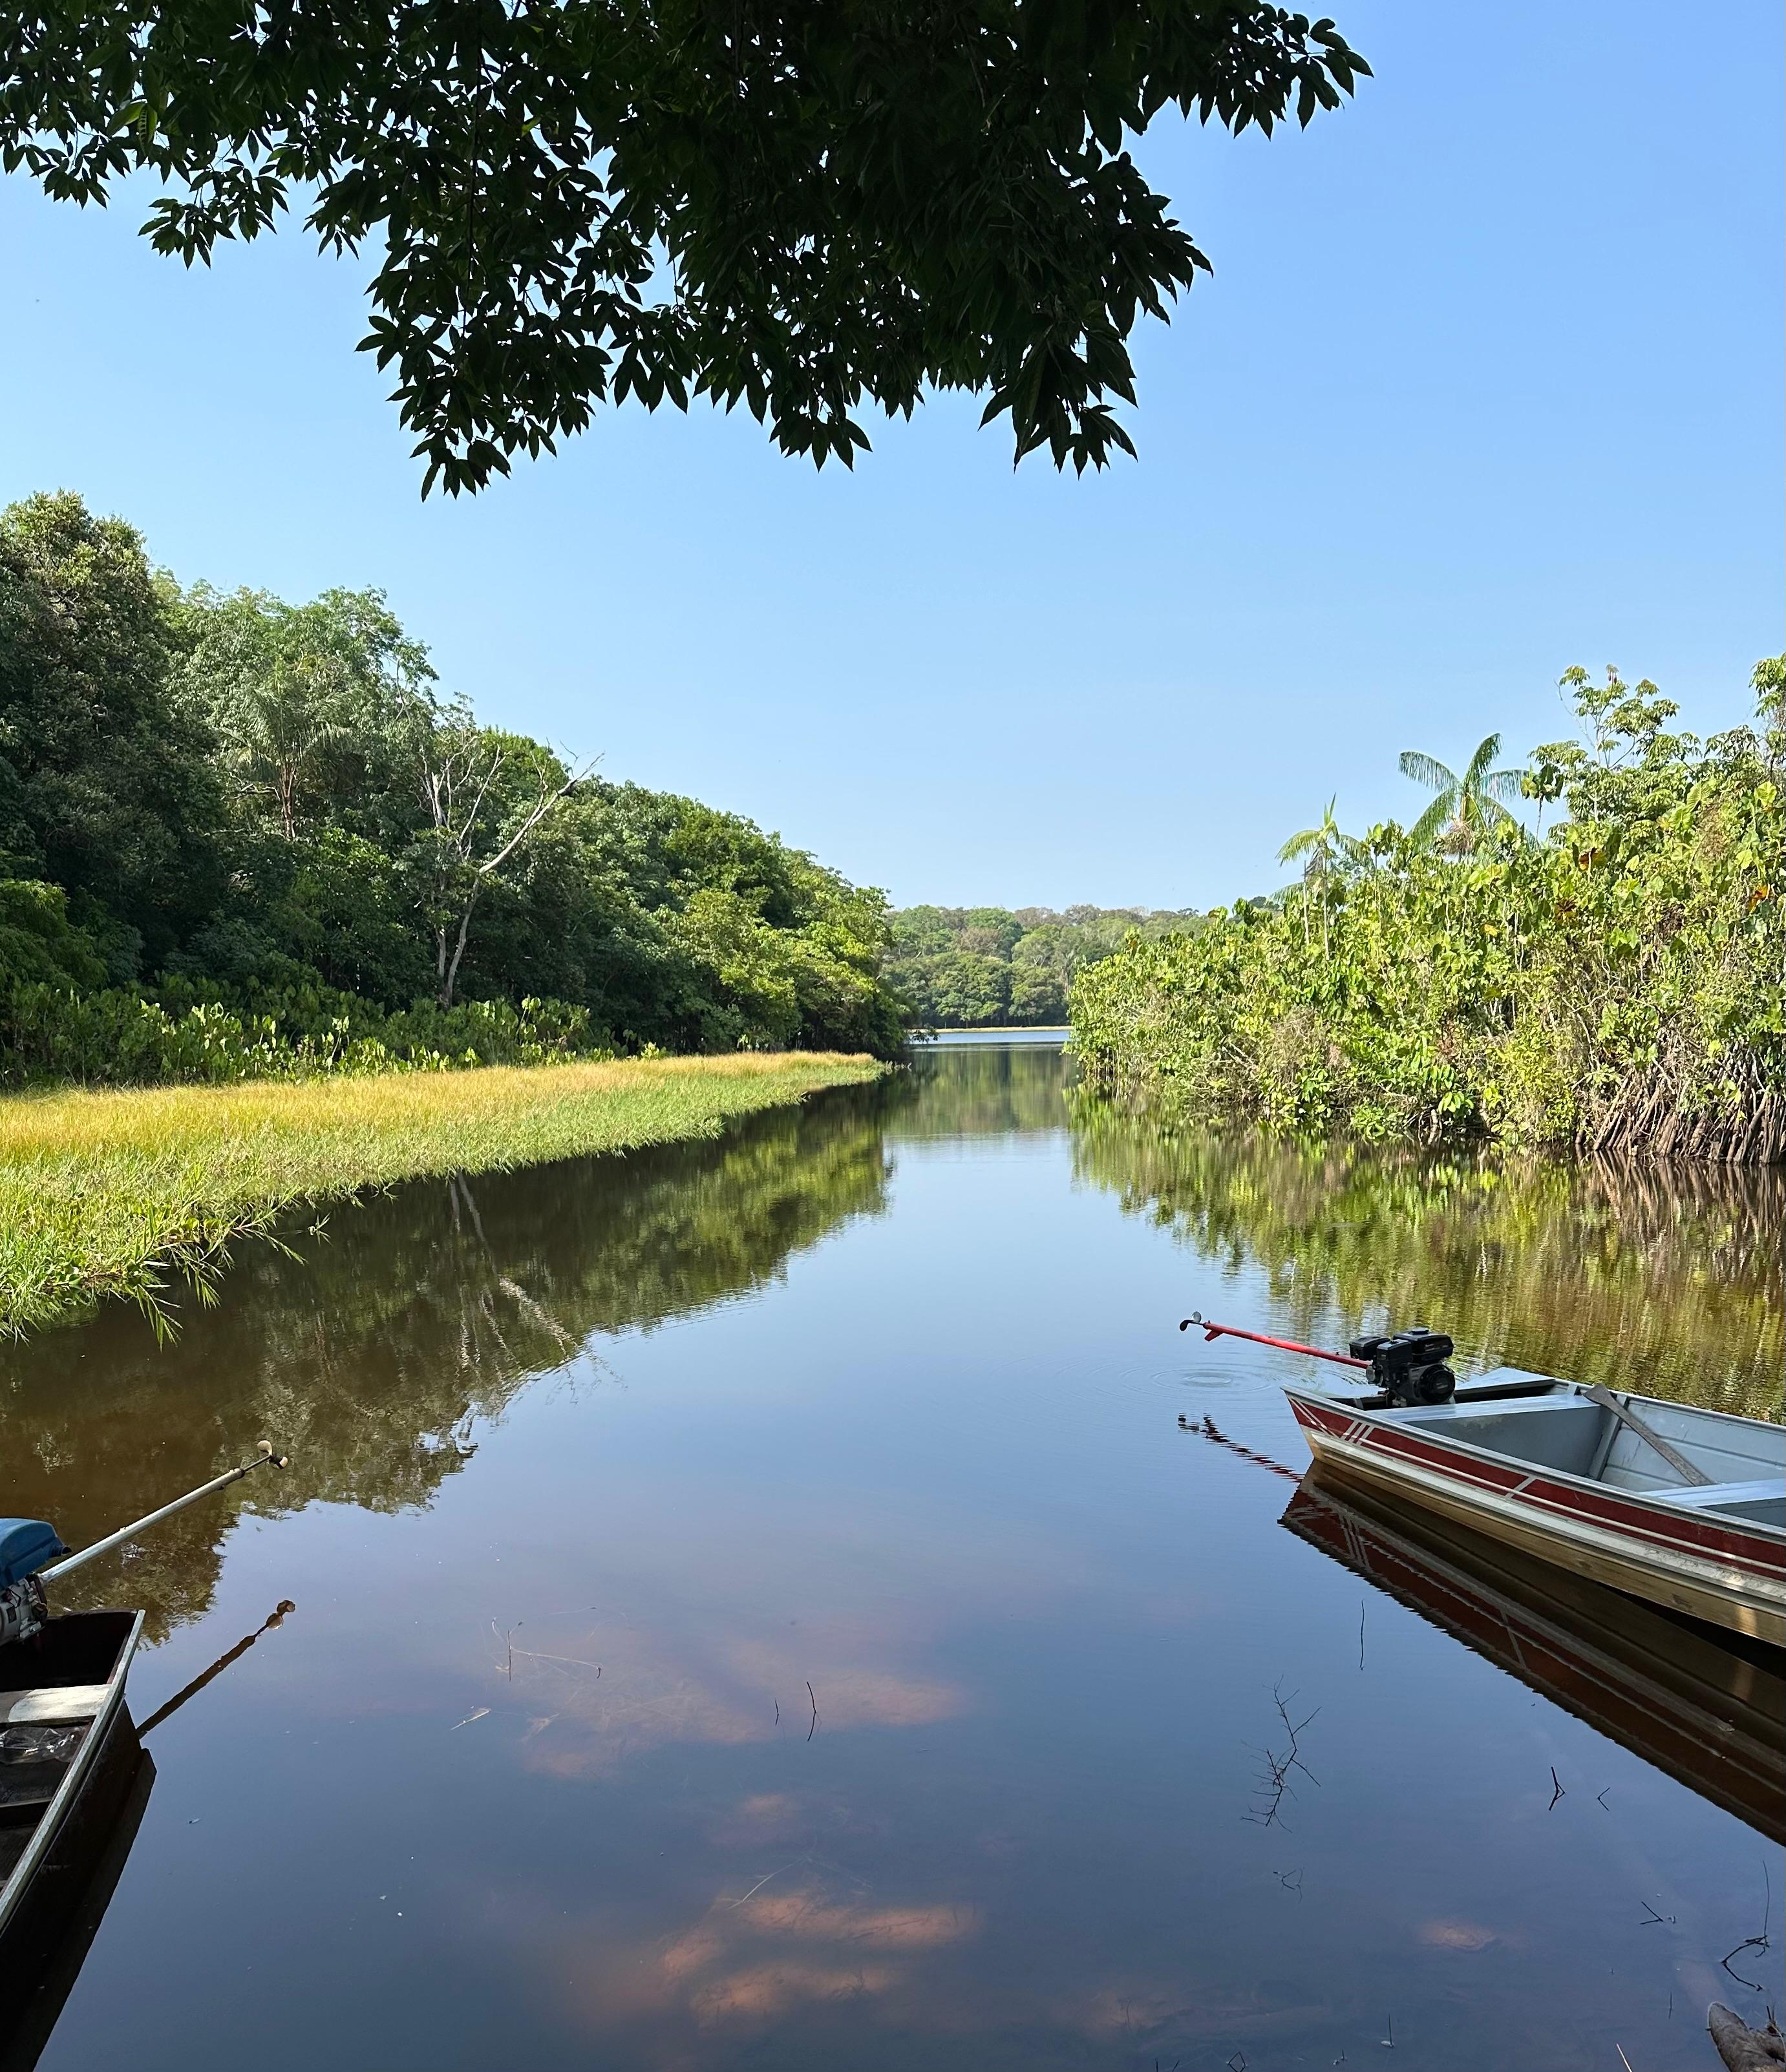
\includegraphics[width=0.4\textwidth]{./artigo/figuras/foto-lago-do-serpa.jpeg}
	\centering
	\caption*{Foto acervo pessoal dos autores, 20/09/2025. }
    \label{fig:minhafigura}
\end{figure}


\FloatBarrier
\subsection{Dados Coletados}

Os dados utilizados nesta pesquisa consistem em parâmetros físico-químicos
coletados in situ no Lago do Serpa, compreendendo as variáveis: pH, oxigênio 
dissolvido (OD), temperatura, cor aparente, cor verdadeira e turbidez, além das 
coordenadas geográficas (UTM). A coleta original foi realizada em 60 pontos 
amostrais distribuídos estrategicamente pelo lago.

Dada a natureza pontual dessas medições e a necessidade de uma base de
dados densa para o trein amento eficaz de redes neurais profundas,
foi aplicada uma técnica de interpolação espacial sobre os 60 pontos
originais. Esse processo gerou uma malha contínua com aproximadamente 3.000 pontos
de dados sintéticos, preservando as características estatísticas e a
distribuição espacial dos fenômenos observados.
Essa abordagem permitiu a criação de um conjunto de dados robusto o
suficiente para a modelagem computacional proposta, superando a limitação
da escassez de dados primários frequentemente encontrada em estudos
ambientais na região amazônica.

\subsection{Treinamento e Validação}

O protocolo de treinamento utilizará a divisão padrão de conjuntos de dados: \(70\%\) 
para o treinamento dos modelos, \(15\%\) para a validação e ajuste de hiperparâmetros 
durante o treinamento, e \(15\%\) reservados exclusivamente para testes finais e avaliação 
de desempenho. Para o treinamento das SNNs, que tradicionalmente enfrentam desafios devido à 
não-diferenciabilidade da função de disparo dos neurônios, será utilizado o método de 
\textit{surrogate gradient} (gradiente substituto). Este método permite a aplicação de 
algoritmos de aprendizado supervisionado baseados em gradiente, como o 
\textit{backpropagation-through-time} (BPTT), aproximando a derivada da função de disparo 
durante a passagem para trás (\textit{backward pass}).

\end{document}
